\section{Optimal Policy Solver with Arbitrary Per-Layer Costs}
% C(i, j, m) is given f_i, b_j, compute b_i in least computational cost, subject to m, according to the per-layer compute and memory costs.

Let us restate the exact problem formulation for a sequence of uniform layers, as studied in Section \ref{sec:2-5-dp-checkpointing}:

\textit{Find the optimal cost }\(C(t,\,m)\)\textit{ for performing backpropagation on a sequence of length }\(t\)\textit{ within }\(m\){ memory slots, using checkpointing.}

How do we generalise this to take into account precise per-layer compute and memory costs?

Let \(\alpha : \{f,\, b\}\times[0,\, N+1] \rightarrow \R^+\) and \(\beta : \{f,\, b\}\times[0,\, N] \rightarrow \Z^+\) be the per-layer forward and backward compute costs and memory costs, respectively, denoted \(\alpha^f_i\) for the computational cost of the \(i^\mathrm{th}\) forward, for example.

We can no longer talk about arbitrary sequences of length \(t\), as each individual subsequence of length \(t\) will have different costs defined by \(\alpha\) and \(\beta\).
Thus the cost function now becomes \(C(i,\, j,\, m;\, \alpha,\, \beta)\), and similarly the policy \(D(i,\, j,\, m;\, \alpha,\, \beta)\).
The parameters \(\alpha\) and \(\beta\) will be omitted for brevity when it is clear from the context what they are.

The exact definition of \(C(i,\, j,\, m;\, \alpha,\, \beta)\) becomes:

\textit{Given }\(f_i\)\textit{ and }\(b_j\)\textit{, the minimal computational cost to perform backpropagation on the segment, that is to compute }\(b_i\)\textit{, within }\(m\)\textit{ remaining memory, using checkpointing.}

To recap what these tensors are, consider the simplified computational graph for backpropagation not including the weights given in Figure \ref{fig:3-comp-graph}, as derived in Section \ref{sec:2-4-2-peak-mem-training}.

\begin{figure}[h]
    \centering
    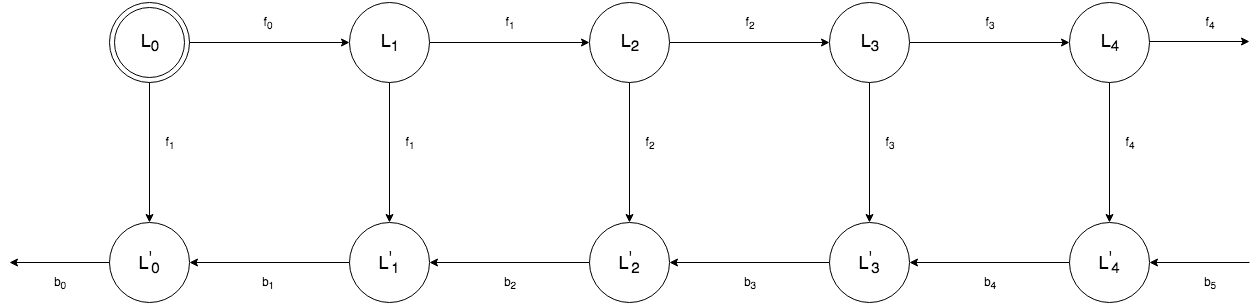
\includegraphics[width=0.95\linewidth]{simplified_comp_graph.png}
    \caption{Computational graph for backpropagation on a sequence, not showing the parameters.}
    \label{fig:3-comp-graph}
\end{figure}

Layer \(i\)'s forward operator takes input \(f_{i-1}\) and produces \(f_{i}\).
Its backward takes \(f_i\) and \(b_{i+1}\) and produces \(b_i\).
\(f_0\) is the inputs and \(b_{N+1}\) is the targets, for an \(N\) layer network.

Now that we have this all defined, we can think about how it affects the solver algorithm.

Iterating over the search space bottom-up no longer means for increasing sequence length \(t\), but over all possible subsequences in `subproblem order' - when we reach the subsequence \((i,\, j)\), we have already solved all \textit{its} subsequences.
We can break this down recursively by saying that for any \(i < k < j\), we have already encountered all subsequences of \((i,\, k)\) and \((k,\, j)\).
Note, given my formulation of the computational graph, only subsequences where \(i < j\) are defined, so \((i,\, i)\) is not a valid subsequence.

\begin{figure}[h]
    \centering
    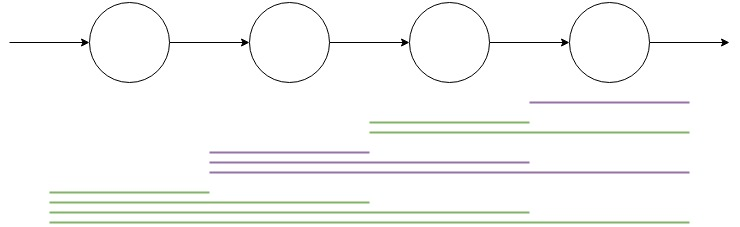
\includegraphics[width=0.75\linewidth]{subproblem-order-traversal.jpg}
    \caption{Visualisation of traversing all subsequences in `subproblem order'. The vertical bars represent a subproblem \((i,\, j)\). Traversal order goes from top to bottom. Notice that, whenever an \((i,\, j)\) is encountered, all of its subproblems have already been done.}
    \label{fig:3-subproblem-order-traversal}
\end{figure}

The way in which I traverse the subsequences is visualised in Figure \ref{fig:3-subproblem-order-traversal}.
For some sequence \((s, e)\), \(i\) and \(j\) start at the end, that is \(i = e-1\) and \(j=e\).
We cannot move \(j\) right.
We have now solved for all subsequences that start with \(i = e-1\).
We move \(i\) left one to \(e-2\) and initialise \(j\) to the first one to the right of \(i\), \(e-1\).
Now, as we move \(j\) further right, we have already done (memoised) all the subproblems \((i^\prime,\, j)\), where \(i^\prime > i\).
In this case, that means we have done all subsequences starting with \(i=e-1\), which is true.
This means that, whenever we are considering a problem \((i,\, j)\), we have already solved all subproblems of \((i,\, i^\prime)\) and \((i^\prime,\, j)\), so never need to go `down' more than one level, but can use the memoised results.
Once we have moved \(j\) all the way right, we have now done all subproblems for \(i \geq e-2\).
Again, we move \(i\) left one to \(e-3\) and initialise \(j\) to \(e-2\).
Once we have solved this case, we move \(j\) right, knowing that we have already solved all \((i,\, i^\prime)\) and \((i^\prime,\, j)\), for all \(i' \geq i\).
We keep traversing like this until eventually we have moved \(i\) left to \(i\), and then \(j\) right to \(e\).

% With all this, Q becomes:
% Q(i,j,k,m) = sum alphas to k + right + left

% however, the fact that we are being precise about memory costs has a large impact on the solution too:

% Because we are no longer using coarse-grained slots, but a specific amount of memory, the solution for some C(i,j,m) does not necessarily use all m memory.
% we want to take advantage of that. If the optimal right and left only use much less memory than the specified m and m_r, we have less pressure to trade-off compute for memory at this `level' of the search space, so have opened up possible solutions with lower comp cost.
% This means, as well as C, we need to track a B(i,j,m) that represents the peak memory within which C(i,j,m) was achieved.
% What, then, is the corresponding peak memory for Q(i,j,k,m)?
% Let us clarify that B(i,j,m) means i,j already in memory, do i,j in m.
% First, we do forwards to k in-place, so the peak mem is the forwards pairwise (not including f_i)
% Second, we do the right hand side in b_r whilst holding f_k, giving f_k+b_r
% Third, we do the left hand side in b_l
% The peak memory for us becomes the max of these three stages
% Actually, given the fact that C(i,j,m) means b_j in memory, this doesn't quite work, but I will address after addressing the case of failure.

% Again, because being precise about memory costs and not using coarse memory slots that all layers can definitely fit into, it is possible for C(i,j,m) to fail because it cannot be done in m memory. 
% e.g. m=50 but the smallest tensor in the segment is 100, so even with constant mem strategy it cannot be done.
% Thus, possibility of failure.
% We encode failure into values of B, that is we check if b_r and b_l are failure before being able to evaluate Q(i,j,k,m)
% Even before that though, we must consider we are no longer always recursing with m-1, but an arbitrary number.
% so, we must check if m_r > 0 too
% if none of these conditions hold for any k, the recursive case fails.

% failure propagation. explain later

% Now, going back to why the calculation of peak memory of Q(i,j,m,k) does not work.
% Use diagrams to show how b_j not being freed.
% Explain gives same problem when we transition from right to left subproblems
% Thus, we must tweak definition of B/C: f_i is computed and already in memory, b_j is computed but must be placed within your m memory.
% In effect, we are propagating down responsibility of placing and freeing b_j to the subcall that will eventually do f_j-1, b_j -> b_j-1

% with all this, algorithm becomes:

% Notice we have done memoisation in the algo we are yet to discuss.
% First, as we go over the k loop, we need cost of f_i->f_k. Obviously, this can be acculumated over the loop so we only have to add f_k each time, not compute the whole f_i to f_k.
% We could memoise this over i too - as in, given cost of forwards from i->k, when we come across i-1->k later, we can do i-1 + i->k.
% However, I don't think the extra effort is worth. The extra code in the j loop is so little compared to the whole loop body that it hardly affects the runtime at all, meaning extra memoisation effort will hardly give any extra effect.
% In fact, I reckon the extra complexity may even make it overall slower.

% Secondly, we can `memoise' failure, that is, propagate failure. If some i,j fails - as in even using the constant memory strategy we cannot do that subsequence - then we definitely cannot do any i',j' where i'<=i, j'>=j. 
% We can propagate this failure right through j easily as we just short-circuit all the j'>=j to failure then break from the j loop.
% Propagating left through i is more complex because i is the outer loop. How would we amend the space of (i,j) iterated over by the loops to remove the (i',j_fail) forall i<=i? The extra complexity probably would in fact increase computational cost and make an already quite unreadable algorithm really unreadable.
% To clarify, I do not mean storing the j_fail at which we failed, then for each i'<i we iterate to, we do the j's up to j_fail then set the rest to fail and break.
% I mean actually skipping over those elements of the search space altogether, like we do by breaking out of the j loop.
% I'm sure any solution would greatly increase complextiy and maybe actually be slower.
% we don't even bother with the stated approach because we would only have to run one extra iteration to j_fail+1 before we hit failure and set all the i,j', j'>=j_fail to failure.

% Next, we still need to address the base cases (constant mem, t=1, constant time)

% t=1 easy, just becomes i=j+1. Set c=, b=. B must *include* j due to updated definition of problem

% constant time? give eqn for peak mem of sequence that does max Bf_i+Bb_i+1 + Bb_i
% However, we need to explicit base case of this. The recursive case and t=1 base case were carefully crafted to account for this themselves: draw diagram explaining how rec case chooses i+1, then, inductively, on the right the rec case chooses i+2, and so on.

% The quadratic case has peak mem of whichever specific f_i->f_k, f_k,b_k+1->b_k, has the highest peak mem. If the peak mem of quadratic > m, we fail
% How to calculate this peak mem efficiently? That is, clearly in the already done subproblems we have already evaulated the peak mem of a lot of the computations that occur in the quadratic case.
% As we iterate from some j-1 to j, most of the quadratic computation is the same, so we should be able to memoise this result to efficiently calculate peak mem for i,j.
% we update a max_per_layer = max(max_per_layer, f_i to f_j, b_j)
%
% Theoretically, we could memoise this properly over all subsequences, not just across the j's for each i. That is, as we go left with i, we could also memoise this peak cost.
% However, this becomes complicated due to the fact that i-1,j modelled i-1 as not in the m memory, whereas i,j models i-1 as in memory. This means we cannot `induct' over the i-1,j possiblity because, if it was the case that i-1,j causes the peak memory, and not some k, k>i-1, then we cannot directly compared the memoised value with the i-1,j case.
% Furthermore, I believe the cost savings of this memoisation would be minimal, considering the memoisation across the j loop only adds a tiny bit of code to an already quite large loop body.
% the extra work involved in working around the above problem may even cause it to be slower!

% Anyway, as for each i, we work out peak per layer cost for quadratic case by memoising over j, the quadratic case becomes a part of the main loop, not some base case we set beforehand.
% So, if the recursive case failed for all k, we use our memoised value to see if quadratic can be done, else we fail for this i,j.

% also, the other j=i+1 base case can just be a part of the main loop too, as we iterate over all subproblems in order. At the top of the i loop, we consider i,i+1 before moving into the j loop for j=i+2...
% Thus, no separate base case loop like in the deepmind algo

% Finally we are done! Full algorithm:
